\documentclass[../main.tex]{subfiles}
\begin{document}
%\chapter{Results}\label{ch:F}
As mentioned in previously, in the course of this thesis we study two trigger Hamiltonians. This chapter focuses on the performance of quantum annealing algorithm upon adding the ferromagnetic trigger, $H_T^F$ (see Eq.~\ref{eq:b13}) to the Ising Hamiltonian. \\
For the same transverse-field initial Hamiltonian, and each problem from the set of problem Hamiltonians, ferromagnetic trigger was added with three different strengths, i.e. the strength parameter, $g$ in Eq.~(\ref{eq:b12}) was chosen to be 0.5, 1 and 2.\\
We begin by studying the dynamics of the same cases as chosen in the previous chapter, to understand the effects of adding the ferromagnetic trigger. In the subsequent sections, the effects of adding the ferromagnetic trigger with different strengths will be discussed. 

\section{The Selected Problems}
We start with problem 733 having a large success probability in case of the original Hamiltonian. Figure~(\ref{fig:f1}) shows the energy spectra for this problem upon adding the ferromagnetic trigger with strengths 0.5, 1 and 2 for all the three annealing times. The corresponding  energy expectation values for the instantaneous state have also been included in these plots. 
\begin{figure}
\centering 
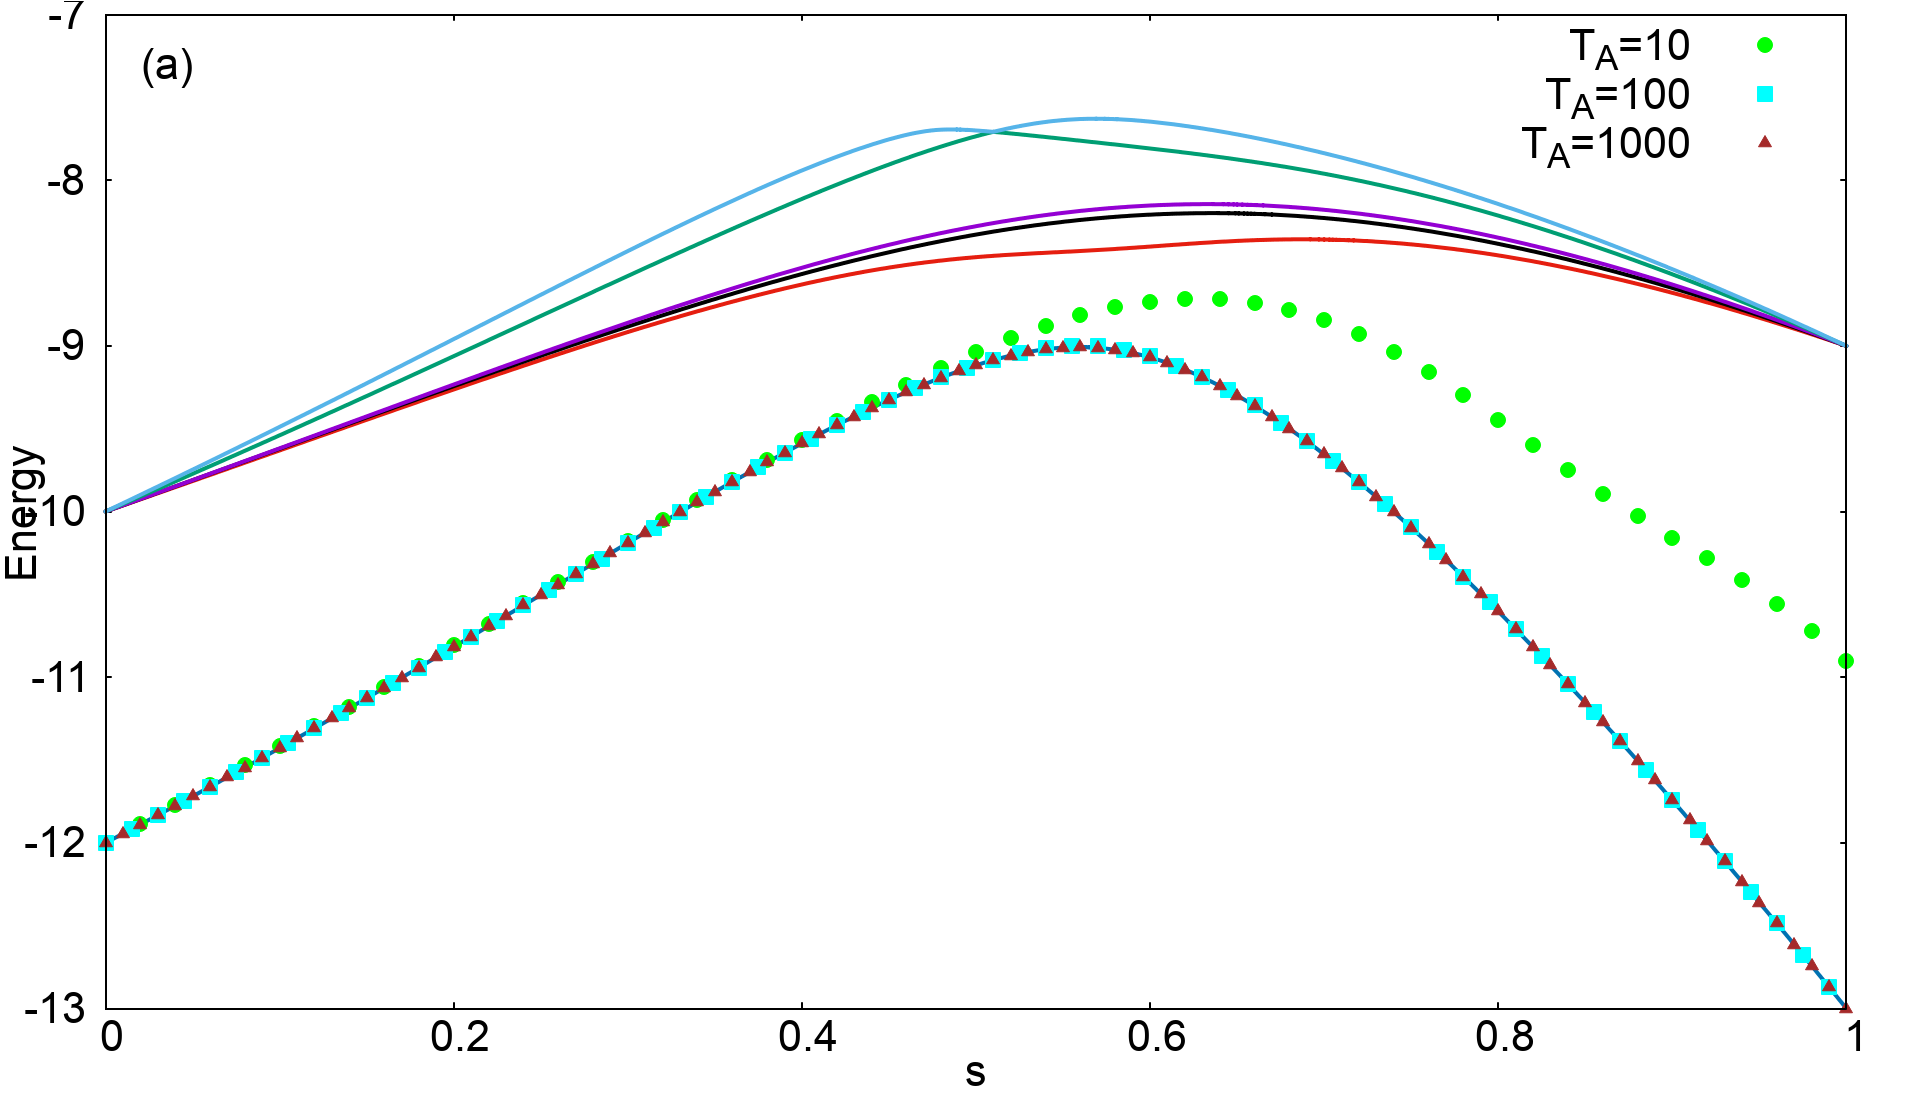
\includegraphics[scale=0.24]{733_s12_F_g0.png}
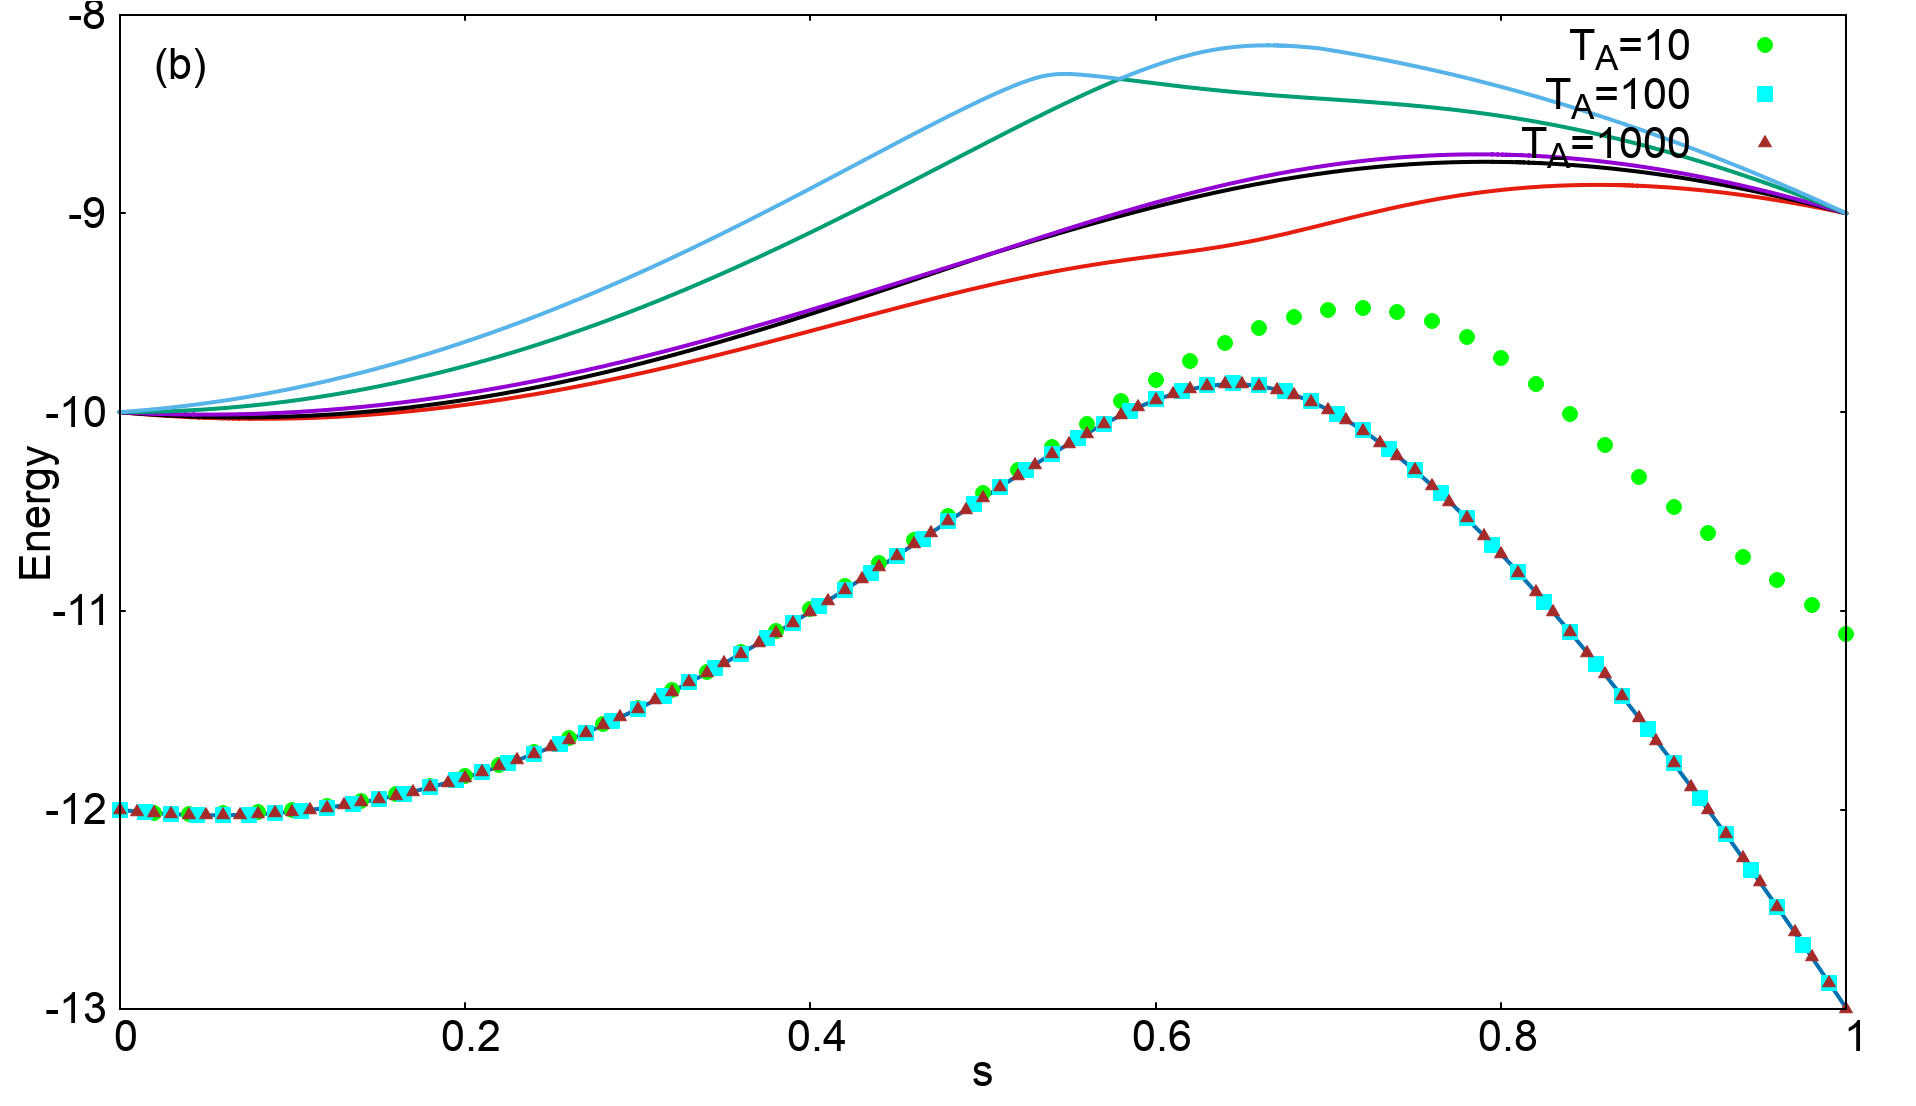
\includegraphics[scale=0.24]{733_s12_F_g1.png}
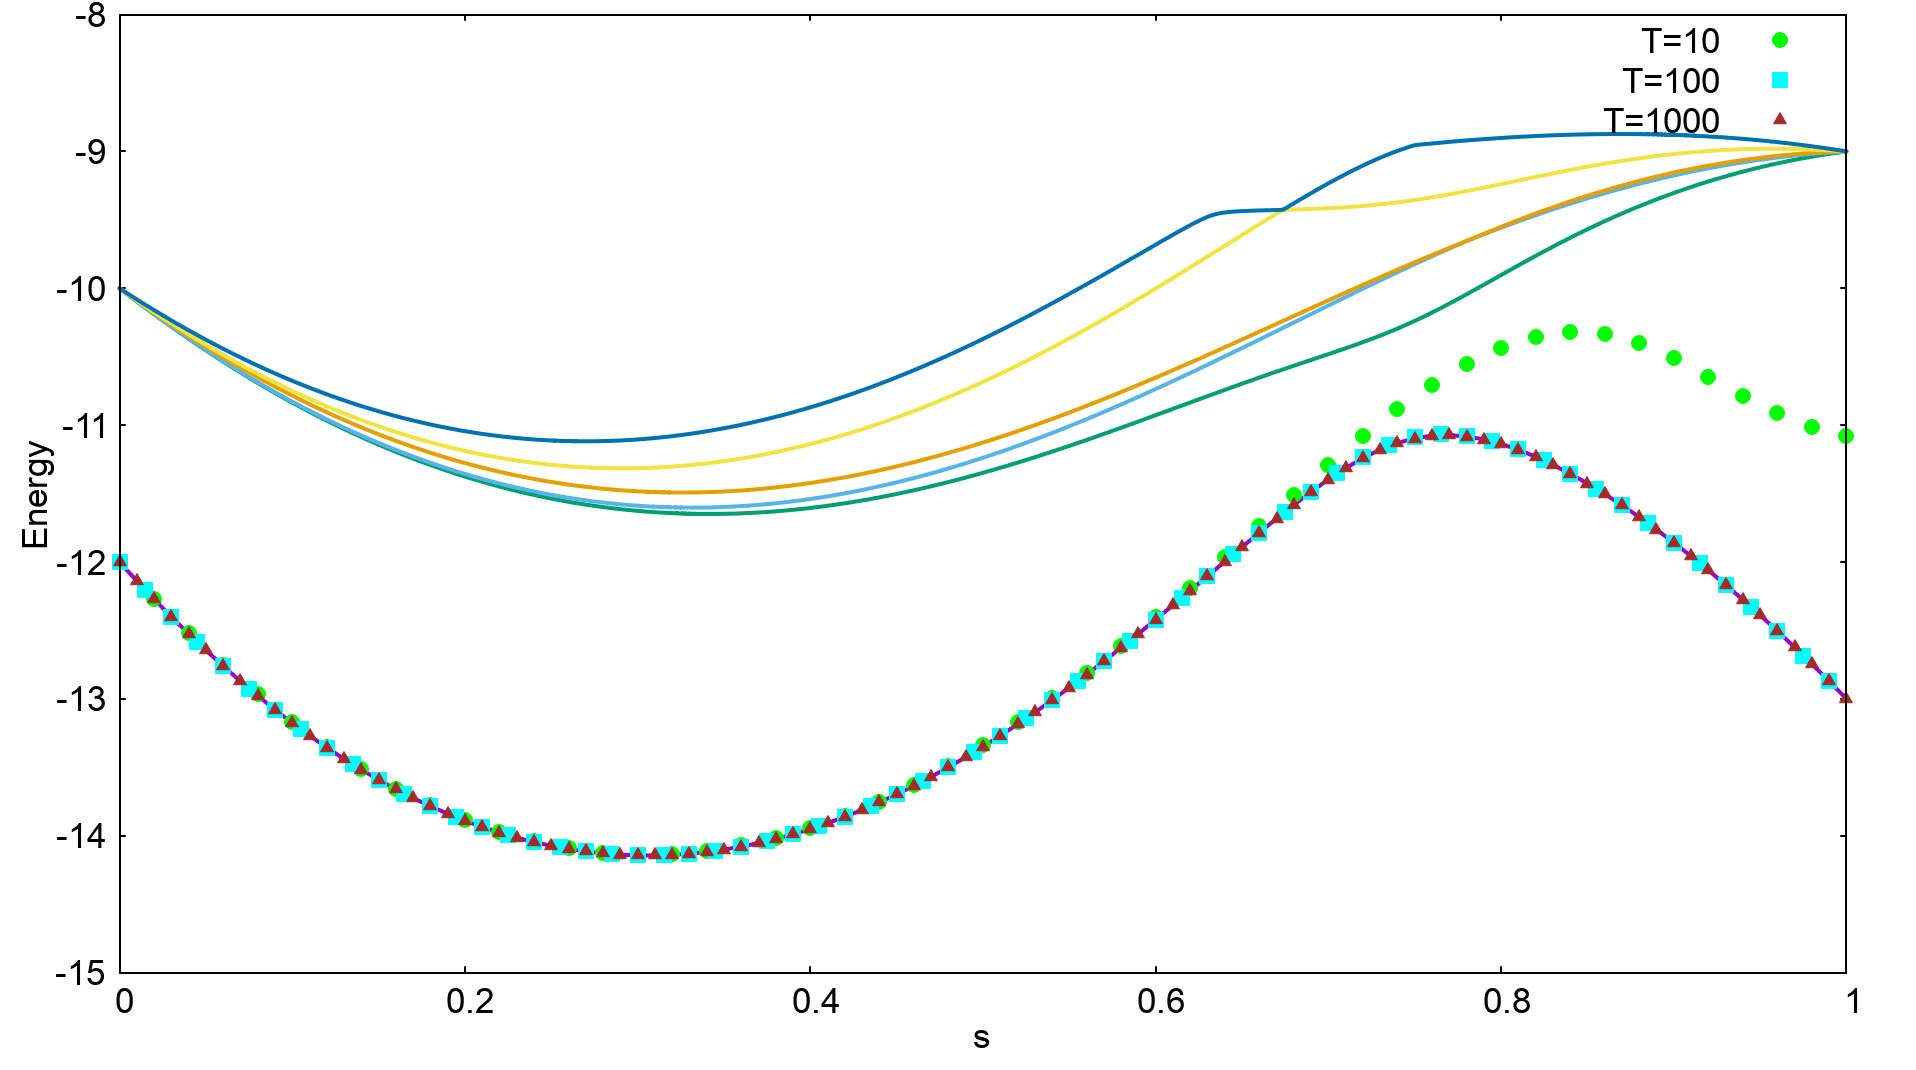
\includegraphics[scale=0.24]{733_s12_F_g2.png}

\caption{The energy spectrum and energy expectation values for the instantaneous state of problem 733, after adding the ferromagnetic trigger. (a): $g$=0.5; (b): $g$=1; (c): $g$=2. }
\label{fig:f1}
\end{figure}

From these figures, it can be noted that compared to the original Hamiltonian, the minimum gap, $\Delta_{min}$ has increased in all the three cases. Furthermore, $\Delta_{min}$ becomes larger as the strength of the trigger Hamiltonian is increased from 0.5 to 2. \\
Secondly, the position of $\Delta_{min}$ is shifted more rightwards upon increasing the strength. 
Moreover, all the success probabilities upon adding the trigger are larger than the success probability of the original Hamiltonian, owing to the increase in the minimum gaps. In general, the success probability also increases with increasing the strength of the trigger, though the final overlap also depends on the the exact energy spectrum. \\
Table~(\ref{tab:f1}) shows a comparison of the minimum energy gaps and success probabilities for problem 733, before and after adding the trigger. 
\begin{table}[H]
\centering
\renewcommand{\arraystretch}{1.3}
\begin{tabular}{|c|c|c|c|c|}
\hline 
Problem 733 & Original Hamiltonian & Trigger=F, $g$=0.5 & Trigger=F, $g$=1 & Trigger=F, $g$=2 \\ 
\hline 
$\Delta_{min}$ & 0.4407 & 0.5779 & 0.6908 & 0.8333 \\ 
\hline 
$p(T_A=10)$ & 0.3444 & 0.4764 & 0.5298 & 0.5222 \\ 
\hline
$p(T_A=100)$ & 0.9944 & 0.9996 & 0.9998 & 0.9997 \\ 
\hline
$p(T_A=100)$ & 0.9999 & 0.9999 & 0.9999 & 0.9999 \\ 

\hline 
value of $s$ at $\Delta_{min}$ & 0.459 & 0.552 & 0.629 & 0.733 \\
\hline

\end{tabular} 
\caption{A comparison of the minimum energy gaps and the success probabilities for $T_A$=100, between the original Hamiltonian for problem 733 and that after adding the ferromagnetic trigger (F) with different strengths. The minimum gaps become larger as the strength of the ferromagnetic trigger is increased. As a result, the success probabilities are increased. The value of $s$ corresponding to the position of the minimum gap also becomes larger.}
\label{tab:f1}
\end{table}

Next, we focus on problem 950, which has a small success probability for the original Hamiltonian. Figure~(\ref{fig:f4})) shows the energy spectra and the energy expectation values for the instantaneous state, upon adding the ferromagnetic trigger with $g$= 0.5, 1 and 2. 
\begin{figure}[H]
\centering 
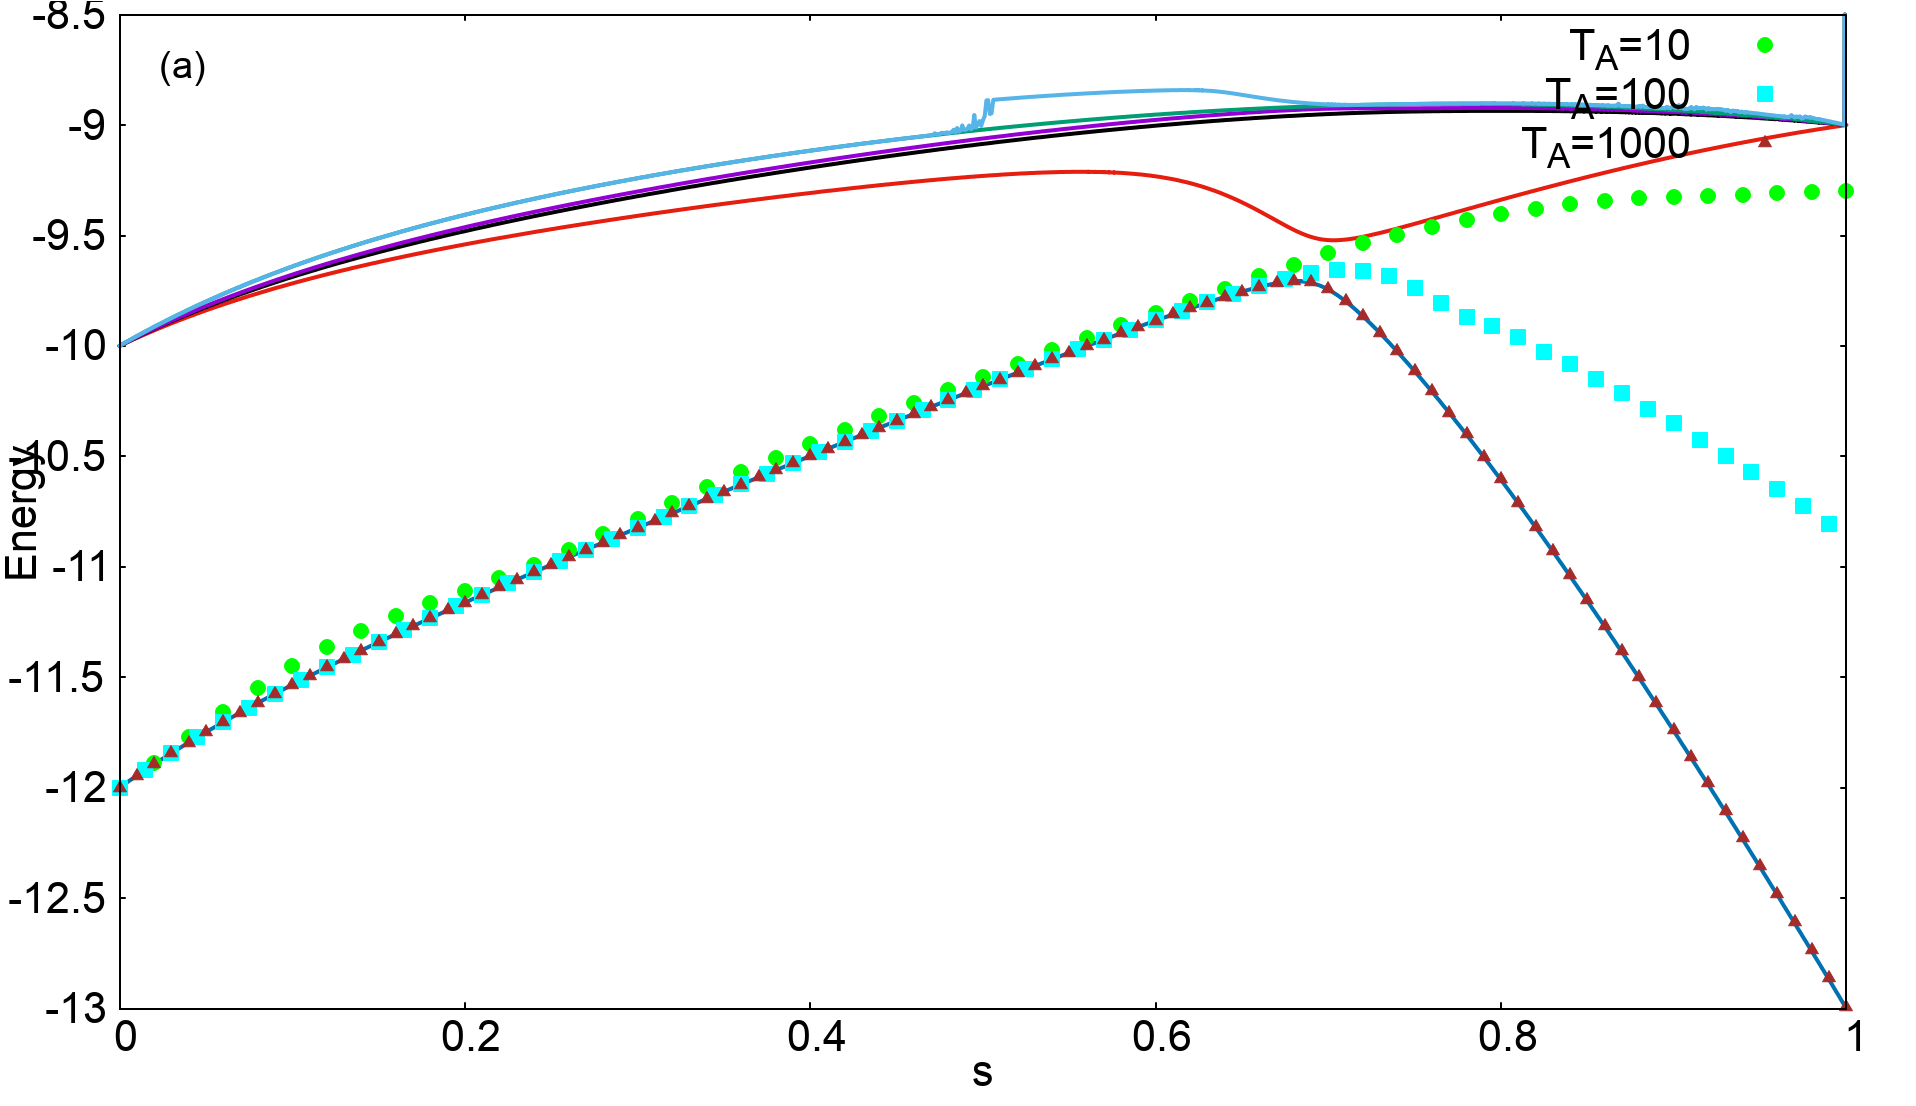
\includegraphics[scale=0.24]{950_s12_F_g0.png}
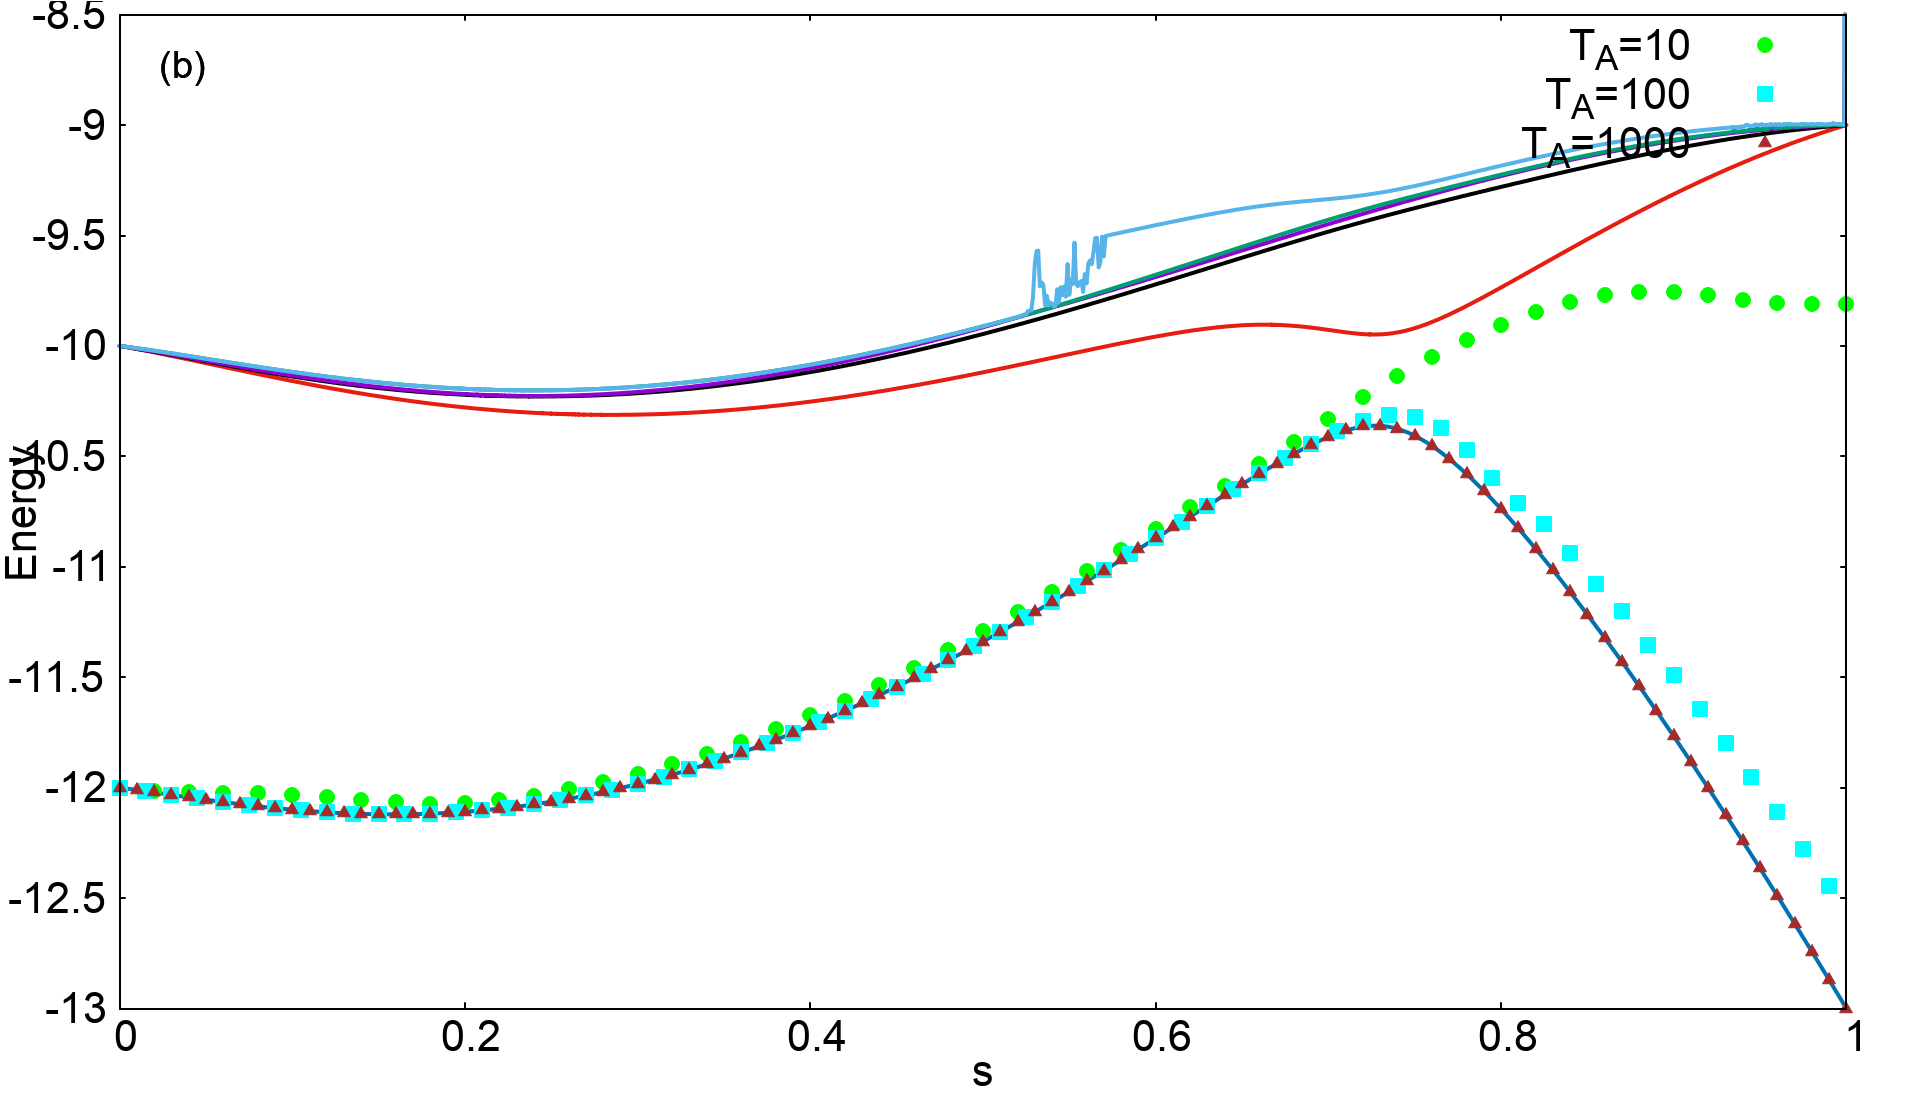
\includegraphics[scale=0.24]{950_s12_F_g1.png}
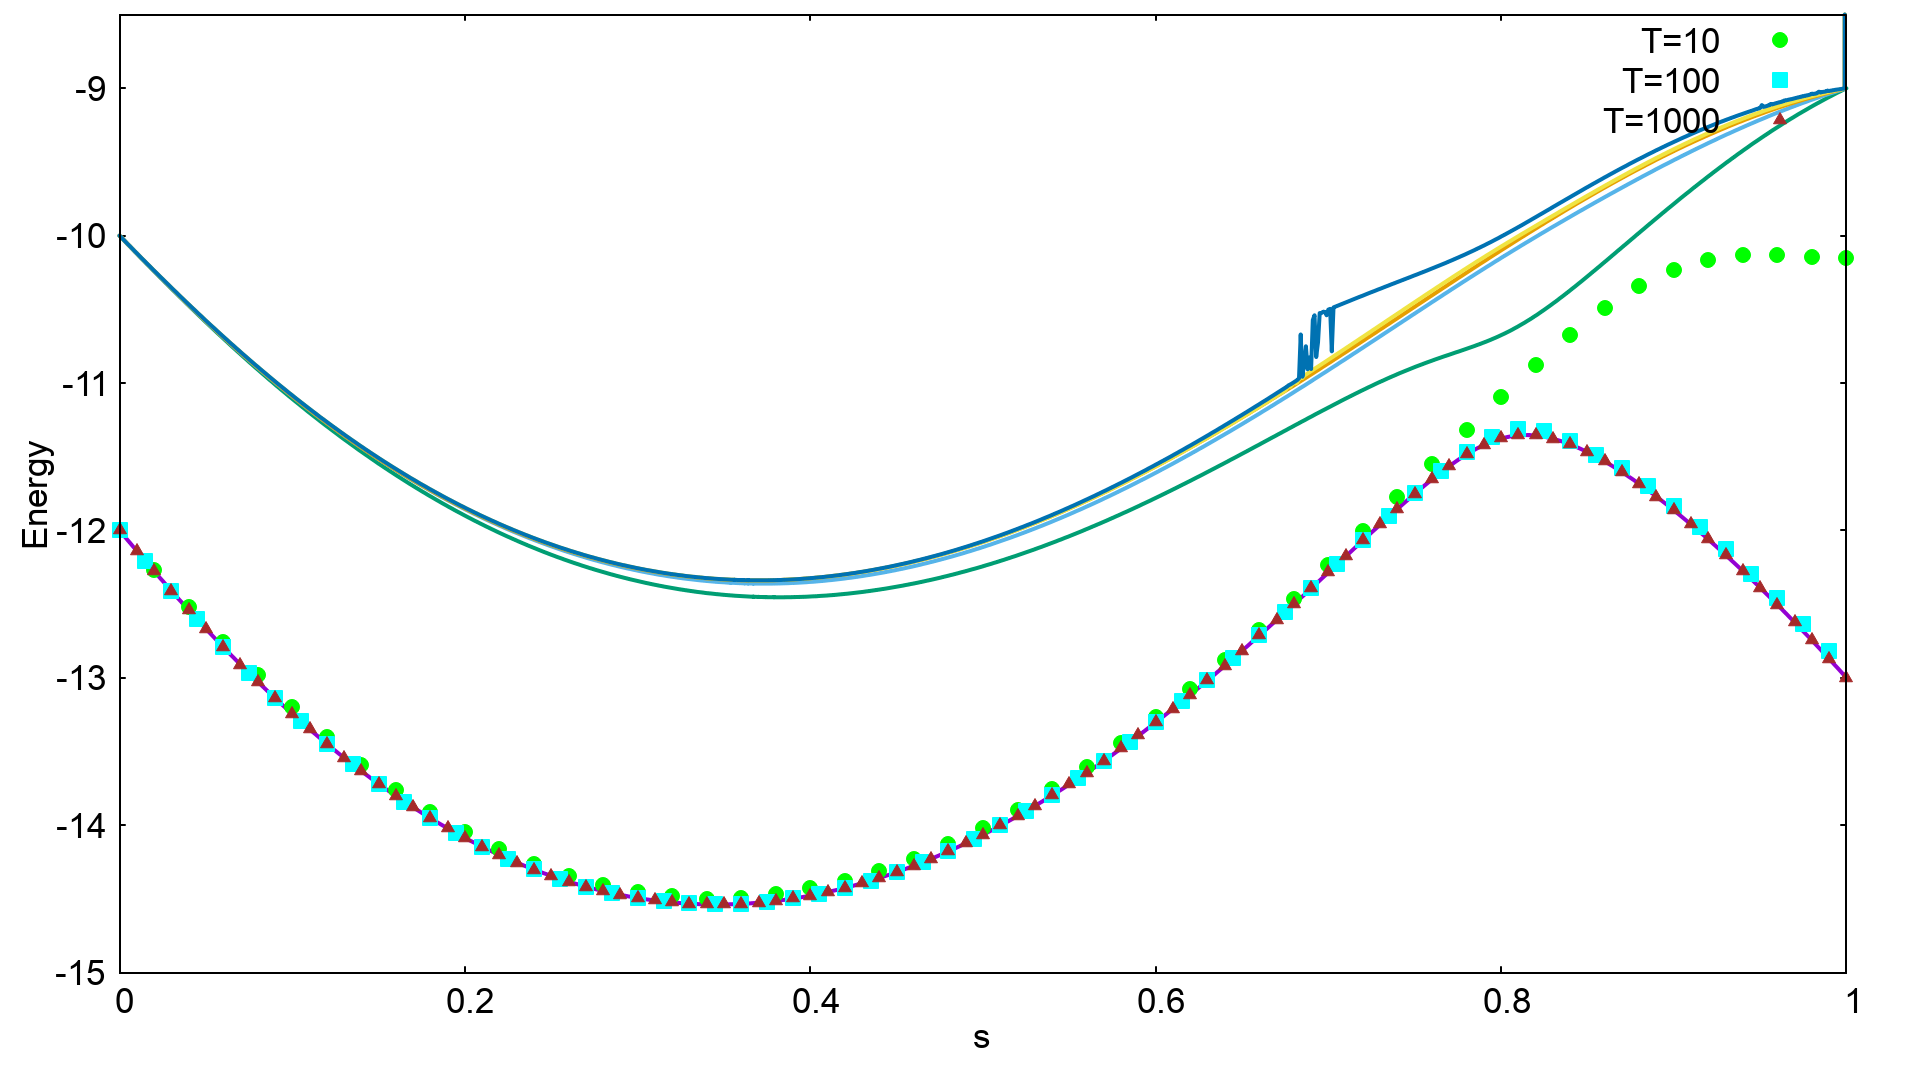
\includegraphics[scale=0.24]{950_s12_F_g2.png}
\caption{The energy spectrum and energy expectation values for the instantaneous state of problem 950, after adding the ferromagnetic trigger. (a): $g$=0.5; (b): $g$=1; (c): $g$=2.}
\label{fig:f4}
\end{figure}
For this case too, the minimum energy gaps increase, leading to an improvement in the success probabilities. The improvements can be seen to become larger with increasing the strength of the trigger. The position of the minimum gap was again found to shift rightwards in terms of the annealing parameter $s$ upon increasing the strength.
However, compared to the improvement in the success probability after adding the ferromagnetic trigger to problem 733, the improvement in problem 950 is significantly larger. Defining the relative success probability as the ratio of the success probability of a particular problem after adding the trigger ($p^F$) to the original success probability ($p^o$), for problem 733, the relative success probability at $T_A$=100 is 1.005 for $g$=2, while that for problem 950 is 67.6. In terms of the ratio of the minimum energy gaps, for problem 733, $\Delta_{min}^F/\Delta_{min}^O$=1.89, while for problem 950, $\Delta_{min}^F/\Delta_{min}^O$=22.2. This can be understood as follows. For the original Hamiltonian in problem 733 and $T_A$=100, the system state always stays close to the ground state of the Hamiltonian (see Fig.~\ref{fig:o2}), because of the large minimum energy gap. Therefore, although adding the ferromagnetic trigger enlarges the minimum gap, there is not much scope for improvement for increasing the overlap with the ground state further. On the other hand, the original minimum energy gap in problem 950 is rather small. This causes the state of the system to shift most of its amplitude to the first excited state, thereby decreasing the overlap with ground state. Since the ferromagnetic trigger widens the minimum energy gap considerably in this case, the overlap with the ground state increases, resulting in a much larger relative success probability. 

In Table~\ref{tab:f2} a comparison of the minimum energy gaps and success probabilities for problem 950, before and after adding the trigger is given.
\begin{table}[H]
\centering
\renewcommand{\arraystretch}{1.3}
\begin{tabular}{|c|c|c|c|c|}
\hline 
Problem 950 & Original Hamiltonian & Trigger=F, $g$=0.5 & Trigger=F, $g$=1 & Trigger=F, $g$=2 \\ 
\hline 
$\Delta_{min}$ & 0.0312 & 0.2074 & 0.4129 & 0.6943 \\ 
\hline 
$p(T_A=10)$ & 0.0002 & 0.0752 & 0.2037 & 0.2914 \\ 
\hline 
$p(T_A=100)$ & 0.0146 & 0.4650 & 0.8889 & 0.9870 \\ 
\hline 
$p(T_A=1000)$ & 0.1362 & 0.9998 & 0.9999 & 0.9999 \\ 
\hline 
value of $s$ at $\Delta_{min}$ & 0.665 & 0.691 & 0.727 & 0.793 \\
\hline

\end{tabular} 
\caption{A comparison of the minimum gaps and the success probabilities for $T_A$=100 between the original Hamiltonian for problem 950 and that after adding the  ferromagnetic trigger with different strengths. The minimum gaps become larger as the strength of the ferromagnetic trigger (F) is increased. As a result, the success probabilities are increased. The value of $s$ corresponding to the position of the minimum gap also becomes larger.}
\label{tab:f2}
\end{table}

Finally, we consider problem 528 with an intermediate success probability for the original Hamiltonian ($g$=0). Figure~(\ref{fig:f7}) shows the energy spectra and energy expectation values for the instantaneous state after adding the ferromagnetic trigger with strengths 0.5, 1 and 2 respectively.

For this case too, the minimum energy gaps increase, leading to an improvement in the success probabilities. The improvements can be seen to have become larger with increasing strengths of the trigger. The position of the minimum gap shifts rightwards in terms of the annealing parameter $s$ upon increasing the strength. \\
The relative success ratio for this case is 1.91 , while $\Delta_{min}^F/\Delta_{min}^O$=4.77 at $g$=2. These values are also intermediate to those for problems 733 and 950. Table~(\ref{tab:f3}) shows a comparison of the success probabilities and the minimum gaps, between the original Hamiltonian ($g$=0) and the Hamiltonian after adding the ferromagnetic trigger with different strengths.
\begin{table}[H]
\centering
\renewcommand{\arraystretch}{1.3}
\begin{tabular}{|c|c|c|c|c|}
\hline 
Problem 528 & Original Hamiltonian & Trigger=F, $g$=0.5 & Trigger=F, $g$=1 & Trigger=F, $g$=2 \\ 
\hline 
$\Delta_{min}$ & 0.1573 & 0.3748 & 0.5439 & 0.7512 \\ 
\hline 
$p(T_A=10)$ & 0.1577 & 0.2959 & 0.4036 & 0.4391 \\
\hline 
$p(T_A=100)$ & 0.5199 & 0.9577 & 0.9945 & 0.9981 \\ 
\hline 
$p(T_A=1000)$ & 0.9999 & 0.9999 & 0.9999 & 0.9999 \\
\hline 
value of $s$ at $\Delta_{min}$ & 0.514 & 0.595 & 0.665 & 0.760 \\
\hline

\end{tabular} 
\caption{A comparison of the minimum energy gaps and the success probabilities for $T_A$=100, between the original Hamiltonian for problem 528 and that after adding the ferromagnetic trigger (F) with different strengths. The minimum gaps become larger as the strength of the ferromagnetic trigger is increased. The success probabilities are increased as a result. The value of $s$ corresponding to the position of the minimum gap also becomes larger.}
\label{tab:f3}
\end{table}
\begin{figure}[H]
\centering 
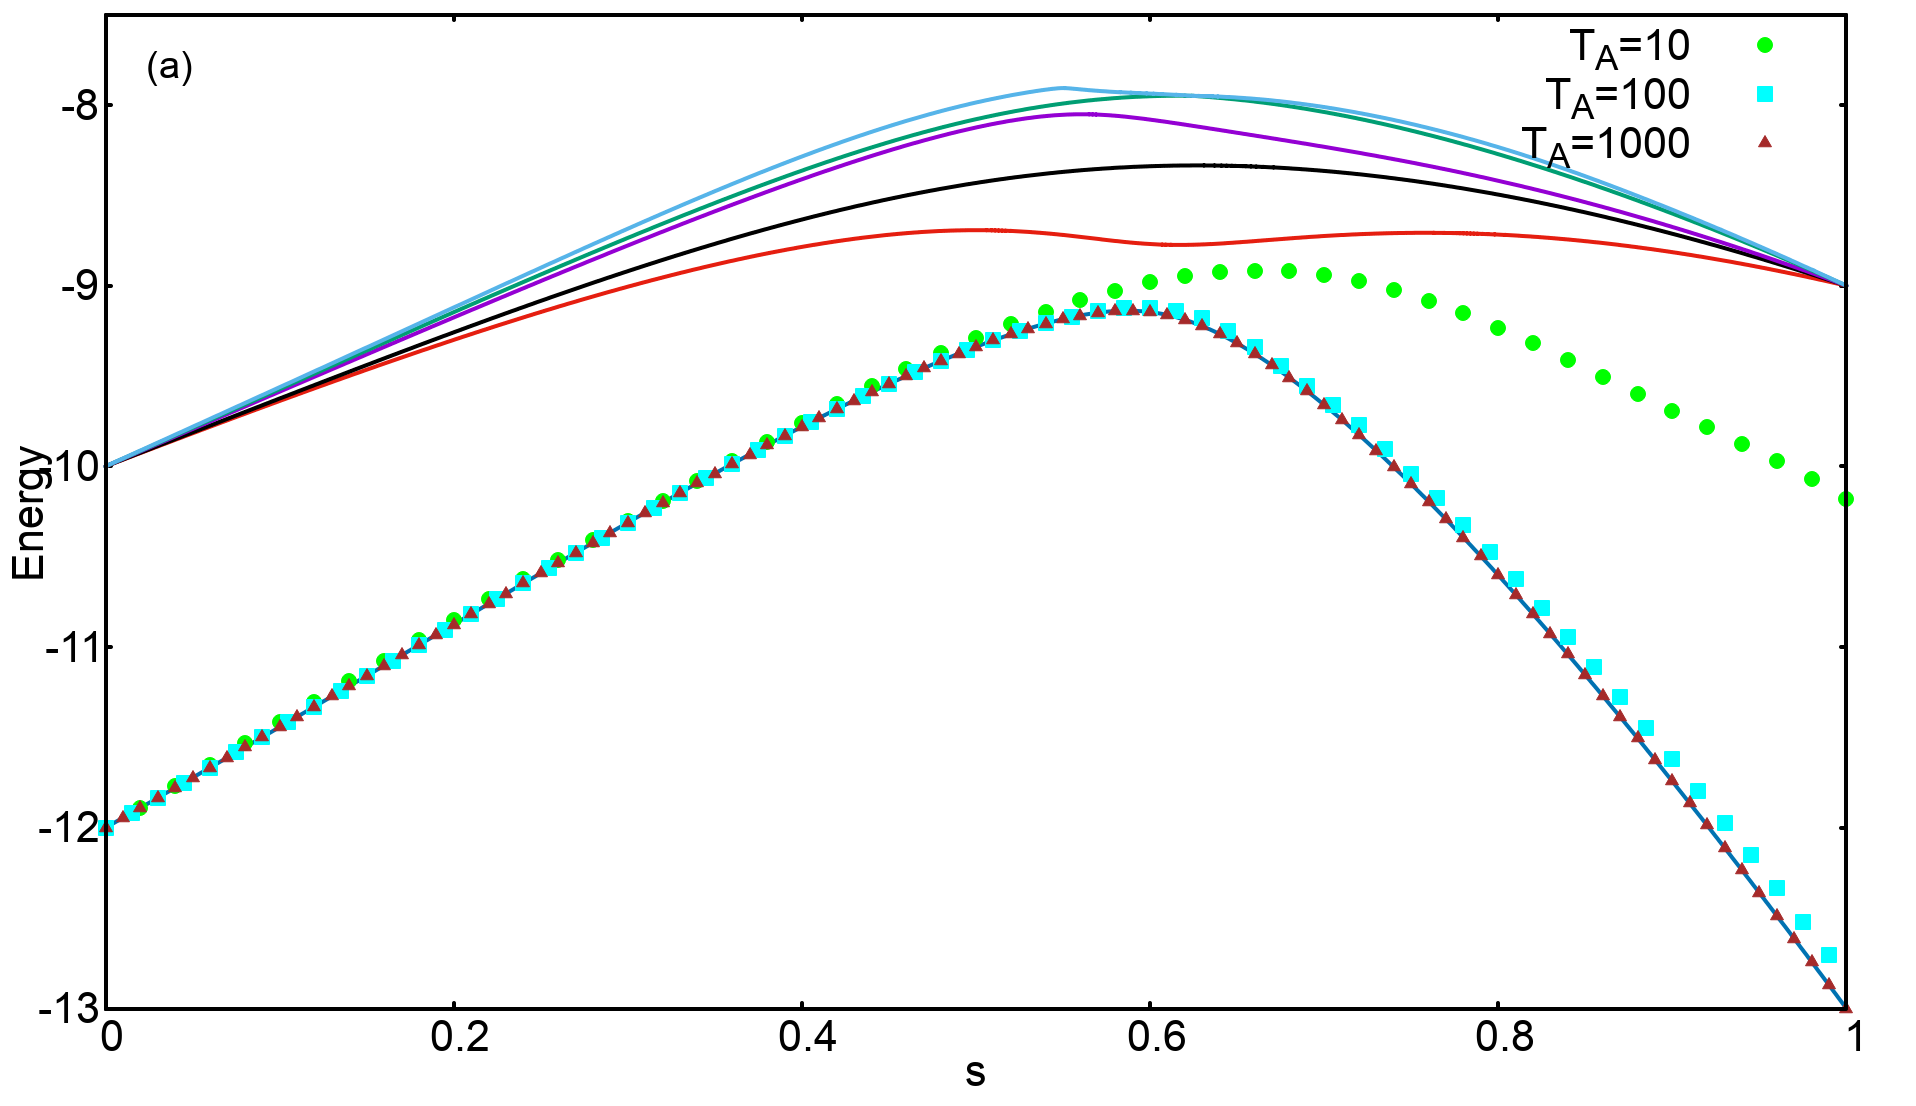
\includegraphics[scale=0.24]{528_s12_F_g0.png}
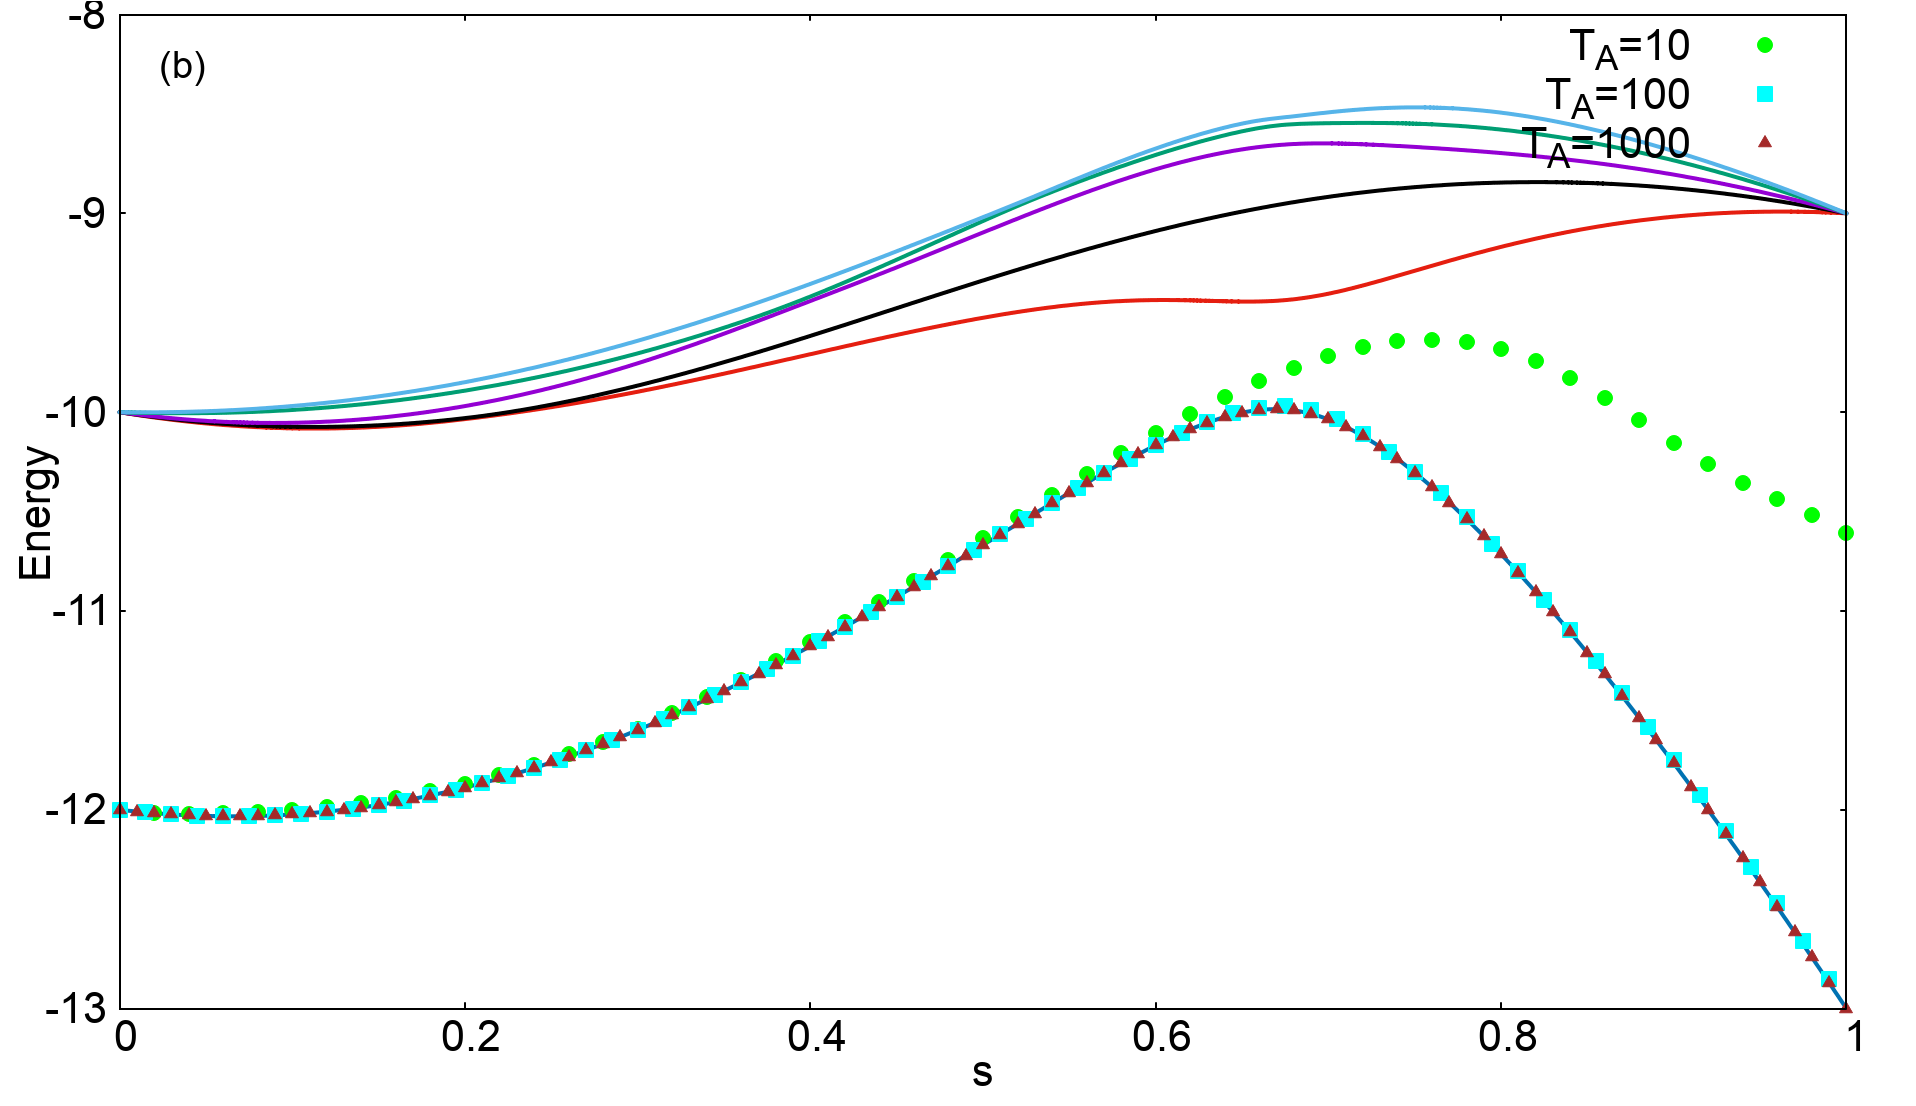
\includegraphics[scale=0.24]{528_s12_F_g1.png}
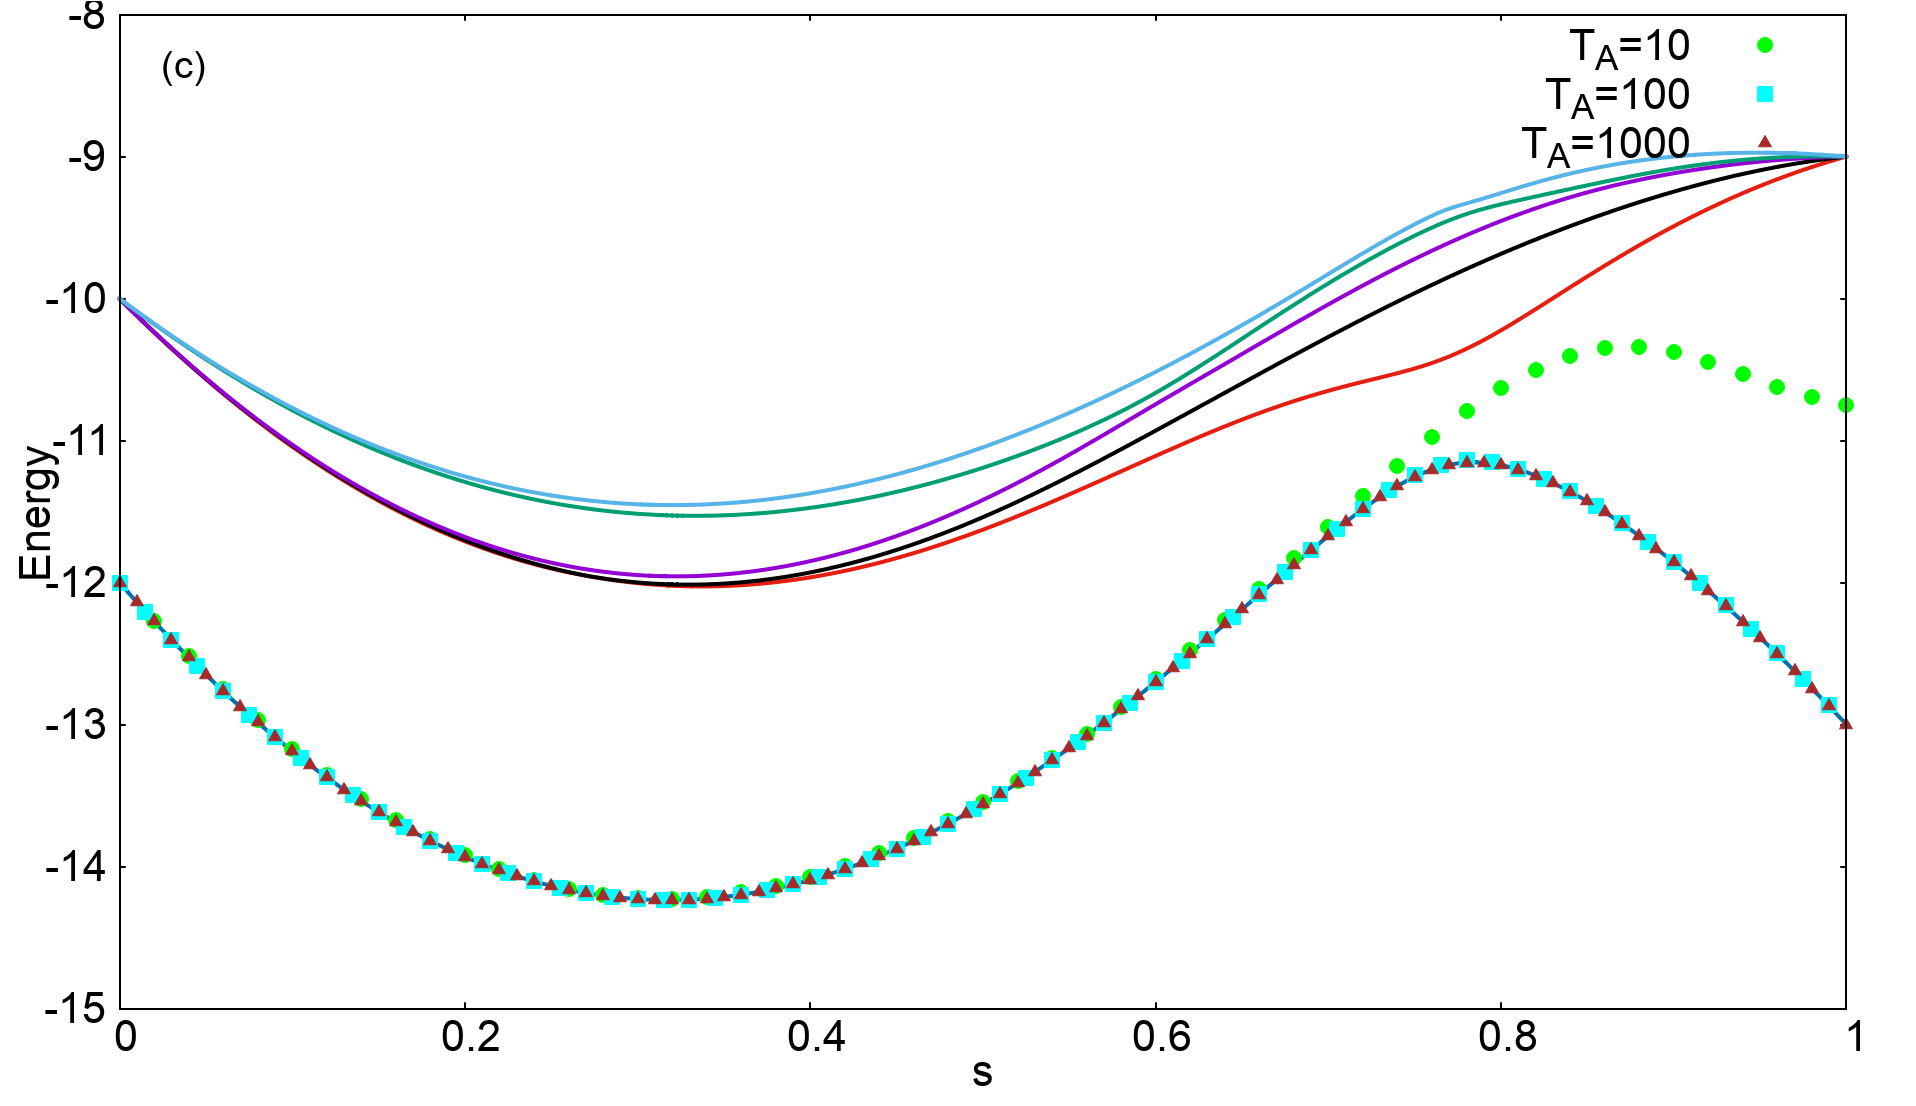
\includegraphics[scale=0.24]{528_s12_F_g2.png}
\caption{The energy spectrum and energy expectation values for the instantaneous state of problem 528, after adding the ferromagnetic trigger. (a): $g$=0.5; (b): $g$=1; (c): $g$=2.}
\label{fig:f7}
\end{figure}

In summary, adding the ferromagnetic trigger enlarges the minimum energy gaps, and the resulting success probabilities are larger than the original success probabilities for all the three problems considered here. The same analysis was then done for all the problems belonging to the set to understand the general effects of adding the ferromagnetic trigger.

\section{The Bigger Picture}
It was observed that the success probabilities after adding the ferromagnetic trigger improve for all the problems of the set, irrespective of the strength of the trigger or the chosen annealing time. To understand the reasons for the same, the minimum energy gaps were computed for all the problems, before and after adding the trigger with $g$ $\in$ \{0.5,1,2\}. \\

Figure~(\ref{fig:f10}) shows the scatter plot of the minimum energy gaps after adding the ferromagnetic trigger with different strengths against the original minimum energy gaps, for all the problems of the set. (The corresponding plot for the problems in the 8-spin set is shown in the appendix as Fig.~\ref{fig:ap1}.)

\begin{figure}[H]
\centering 
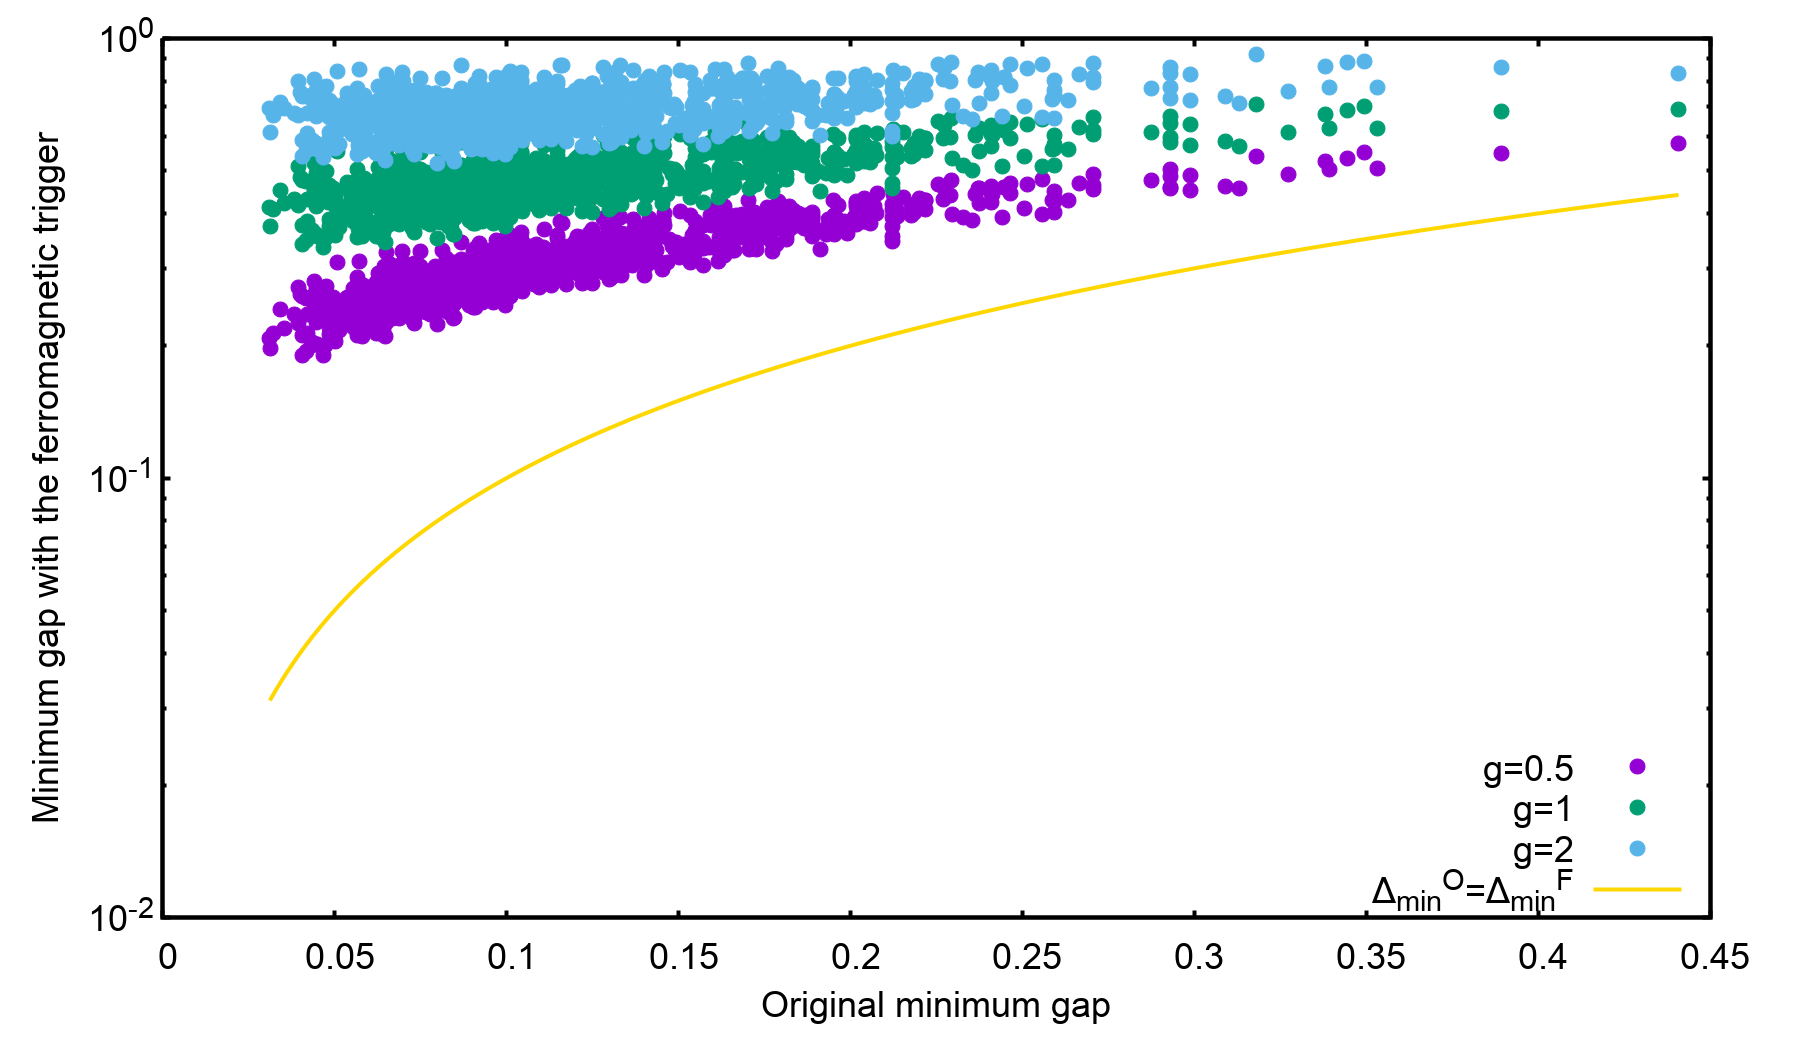
\includegraphics[scale=0.2]{Mingap_F_g0_1_2.png}
\caption{Scatter plot of the minimum gaps upon adding the ferromagnetic trigger with $g$ $\in$ \{0.5,1,2\} against the original minimum energy gaps. The points lying above solid line represent the cases with enlarged minimum gaps.}
\label{fig:f10}
\end{figure}
With the ferromagnetic trigger, all the minimum energy gaps are increased, for  all the values of $g$. Furthermore, for all the problems, the gaps become even larger as the ferromagnetic trigger becomes stronger. It can also be noted that the enhancement in the minimum energy gaps is larger in cases with relatively small original minimum gaps, as was also seen by calculating $\Delta_{min}^F/\Delta_{min}^O$ for the three chosen problems (733, 950 and 528). 

For gauging the performance of the quantum annealing algorithm after adding the ferromagnetic trigger, scatter plots of the success probabilities after adding the ferromagnetic trigger against the original success probabilities have been shown in Fig.~(\ref{fig:f11}) corresponding to $g$=0.5, 1 and 2. (See Fig.~\ref{fig:ap3} for the corresponding plot for the 8-spin problems.)
\begin{figure}[H]
\centering 
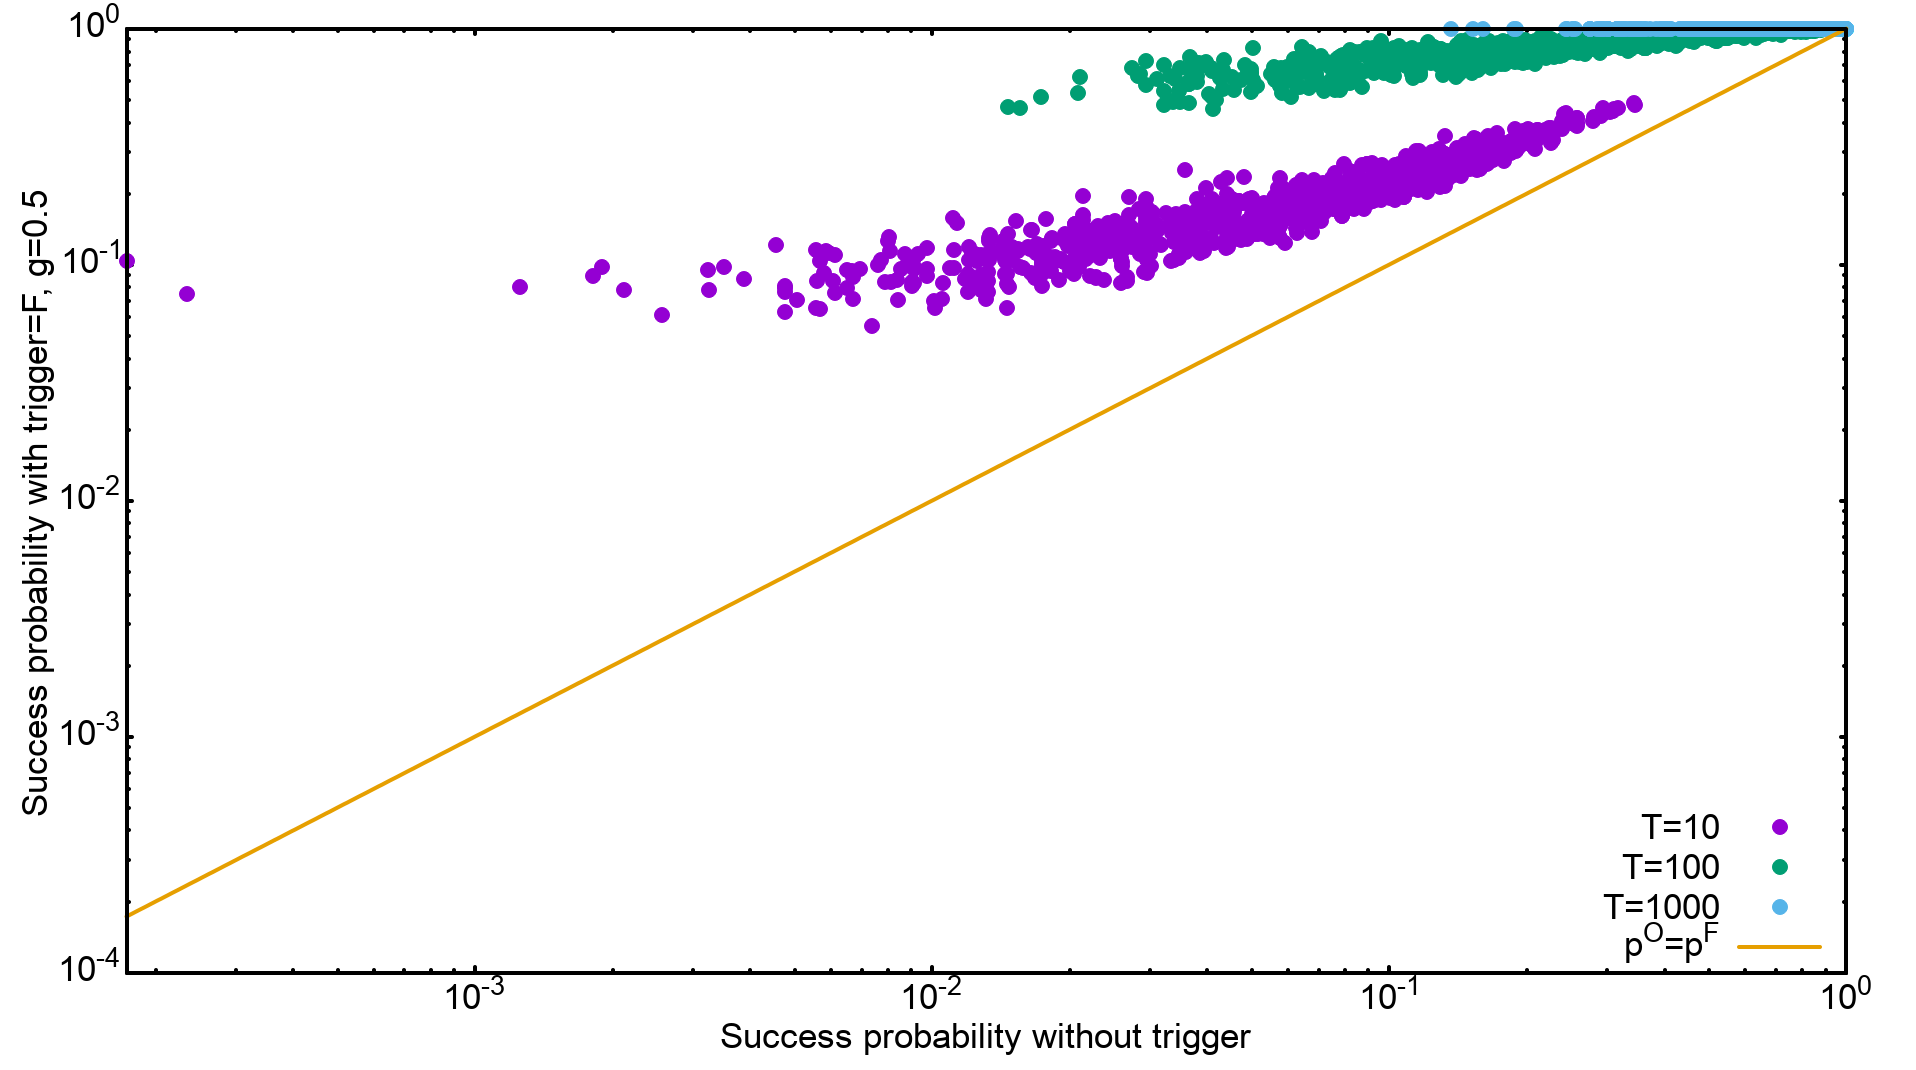
\includegraphics[scale=0.24]{Scatt_s12_F_g0.png}
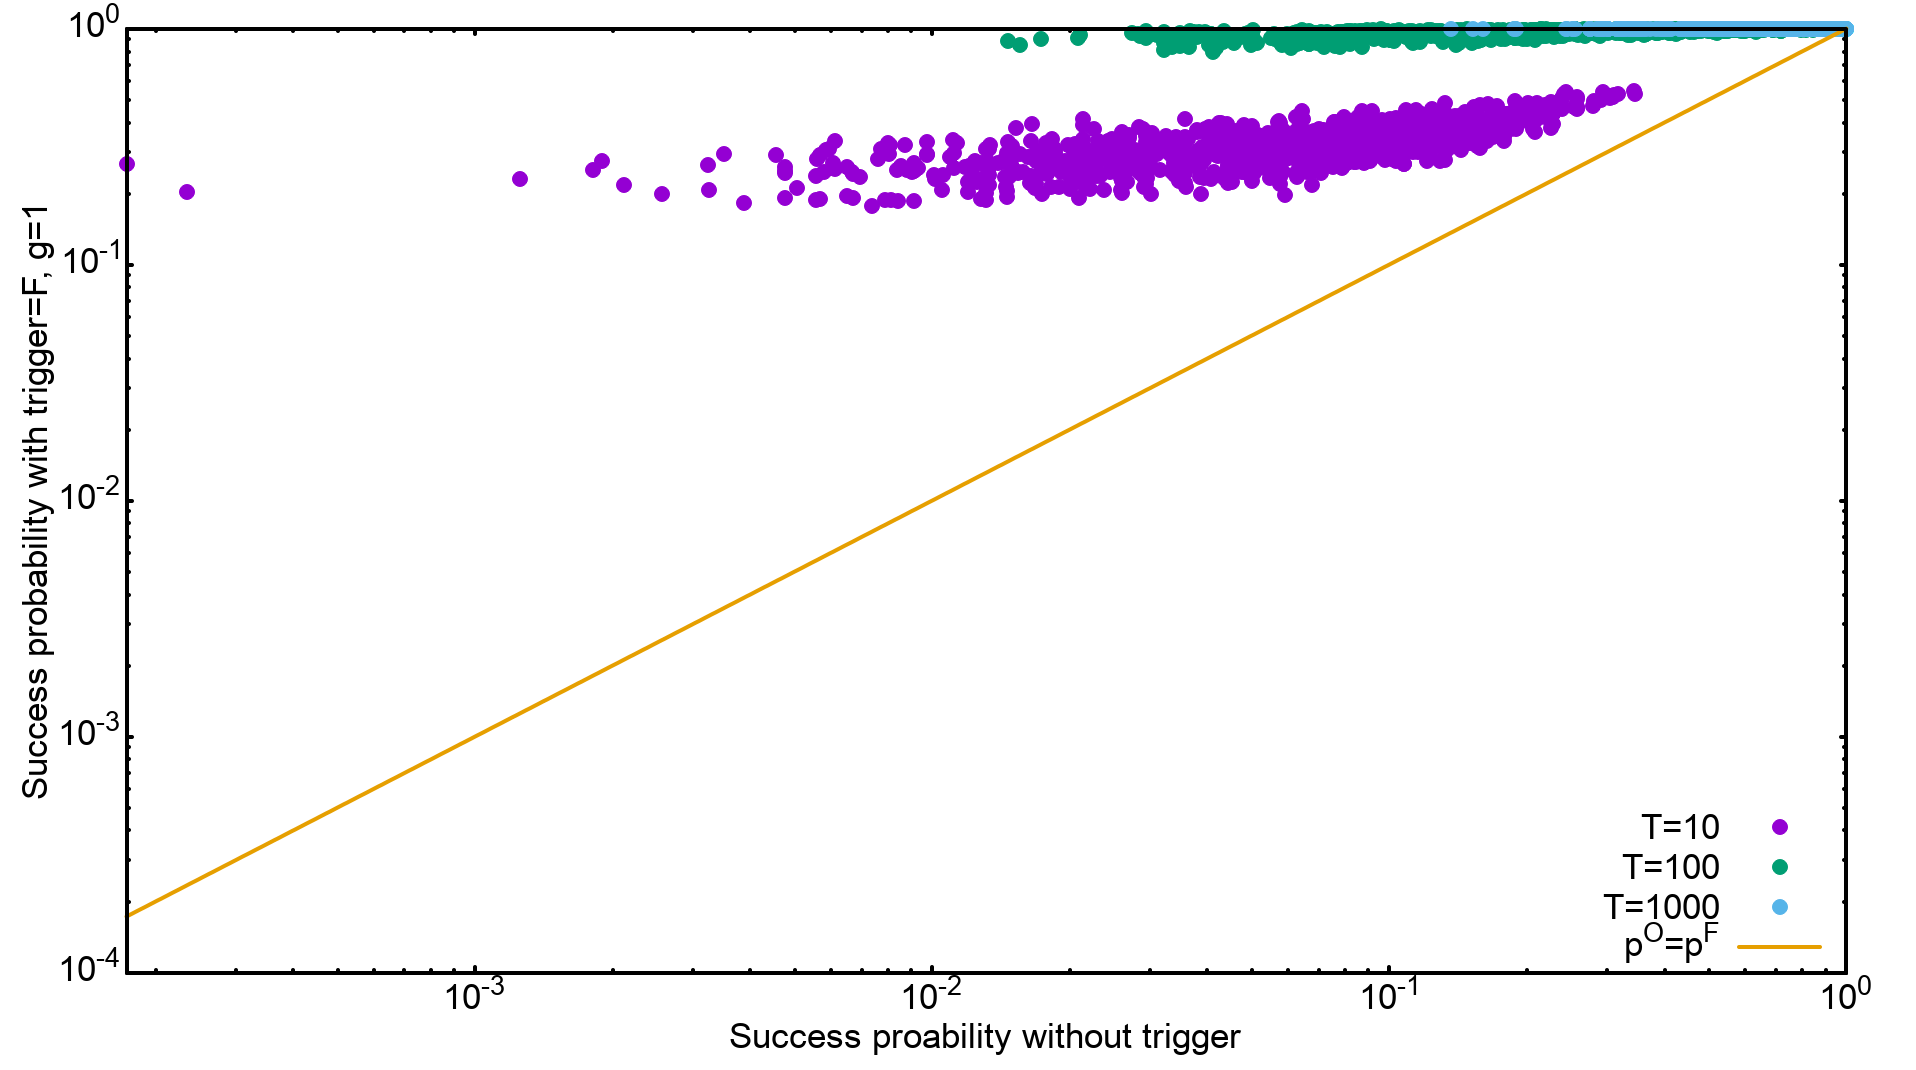
\includegraphics[scale=0.24]{Scatt_s12_F_g1.png}
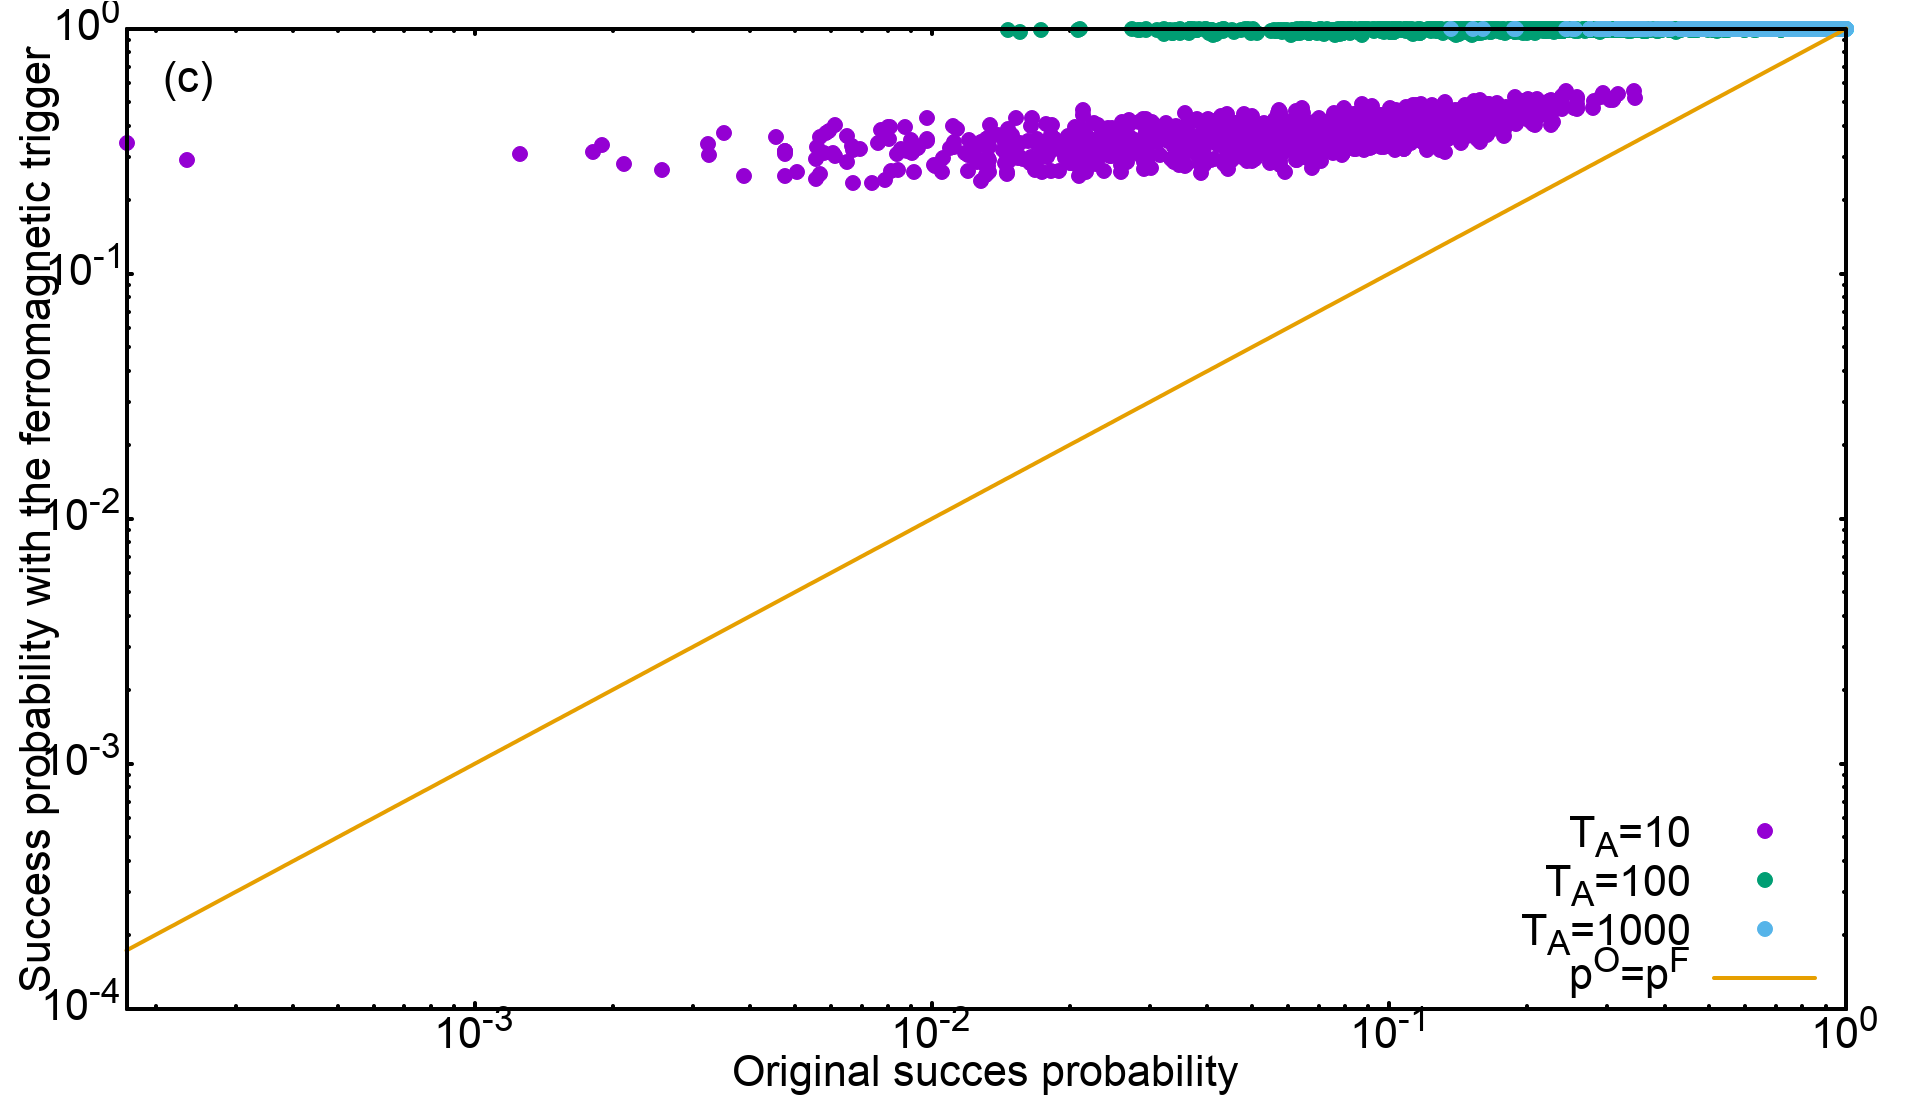
\includegraphics[scale=0.24]{Scatt_s12_F_g2.png}
\caption{Scatter plot for the success probability after adding ferromagnetic trigger against the success probability of the original Hamiltonian, for annealing time $T_A \in \{10,100,1000\}$. (a): $g$=0.5; (b): $g$=1; (c): $g$=2. Points lying above the solid line represent the problems with improved success probability.}
\label{fig:f11}
\end{figure}


For all the three cases, and all the problems in the set, the success probability after adding the trigger is greater than the success probability of the original Hamiltonian. Since in the adiabatic regime, the overlap of the final state with the ground state increases with increasing annealing times, the success probability of the original Hamiltonians for long annealing times ($T_A$=1000) is already large ($\approx$ 1). Adding the ferromagnetic trigger can therefore not improve the success probability too much. This explains the confinement of the points representing the success probability for $T_A$=1000 close to the solid line ($p^O=p^F$) on the upper right corner, for all the three values of the strength parameter. Owing to the same reason, the points corresponding to the success probability for $T_A$=10 have a much larger spread. For the easy cases (larger $p^O$), the success probability upon adding the trigger ($p^F$) has a similar value. Such points lie close to the line. On the other hand, for more difficult cases (smaller $p^O$) the improvement can be larger, and such points lie away from the line.\\

Furthermore, since for a given problem, increasing the strength of the ferromagnetic trigger makes the minimum gaps larger, the success probability for that case also becomes larger. This explains the distribution of the points getting successively more flat with increasing strength of the trigger, for all annealing times (see Fig.~\ref{fig:f11}).\\

Finally, we look at the dynamics of the evolution. According to Eq.~(\ref{eq:lz5}), for an adiabatic evolution of the state of the system, the success probability, $p$, which is a measure of the overlap of the final state with the ground state of the Hamiltonian, is related to the minimum energy gap, $\Delta_{min}$ as follows:
\begin{equation}
p=1-\exp(-C{\Delta_{min}}^2),
\end{equation}
for some constant $C$. Since different problems belonging to the set may correspond to different minimum energy gaps, a plot of the success probability with these gaps should follow Eq.~(\ref{eq:lz5}) if the evolution of the state for a problem is adiabatic. Moreover, adding the trigger changes the energy spectra, and thereby the minimum energy gaps of these problems. Figure~(\ref{fig:f14}) shows the success probability versus the minimum energy gap plot for all the problems upon adding the ferromagnetic trigger with three different strengths (0.5,1 and 2), and for three annealing times (10,100 and 1000). (See Fig.~(\ref{fig:ap5}(a)) for the corresponding plot for 8-spin problems.)

\begin{figure}[H]
\centering
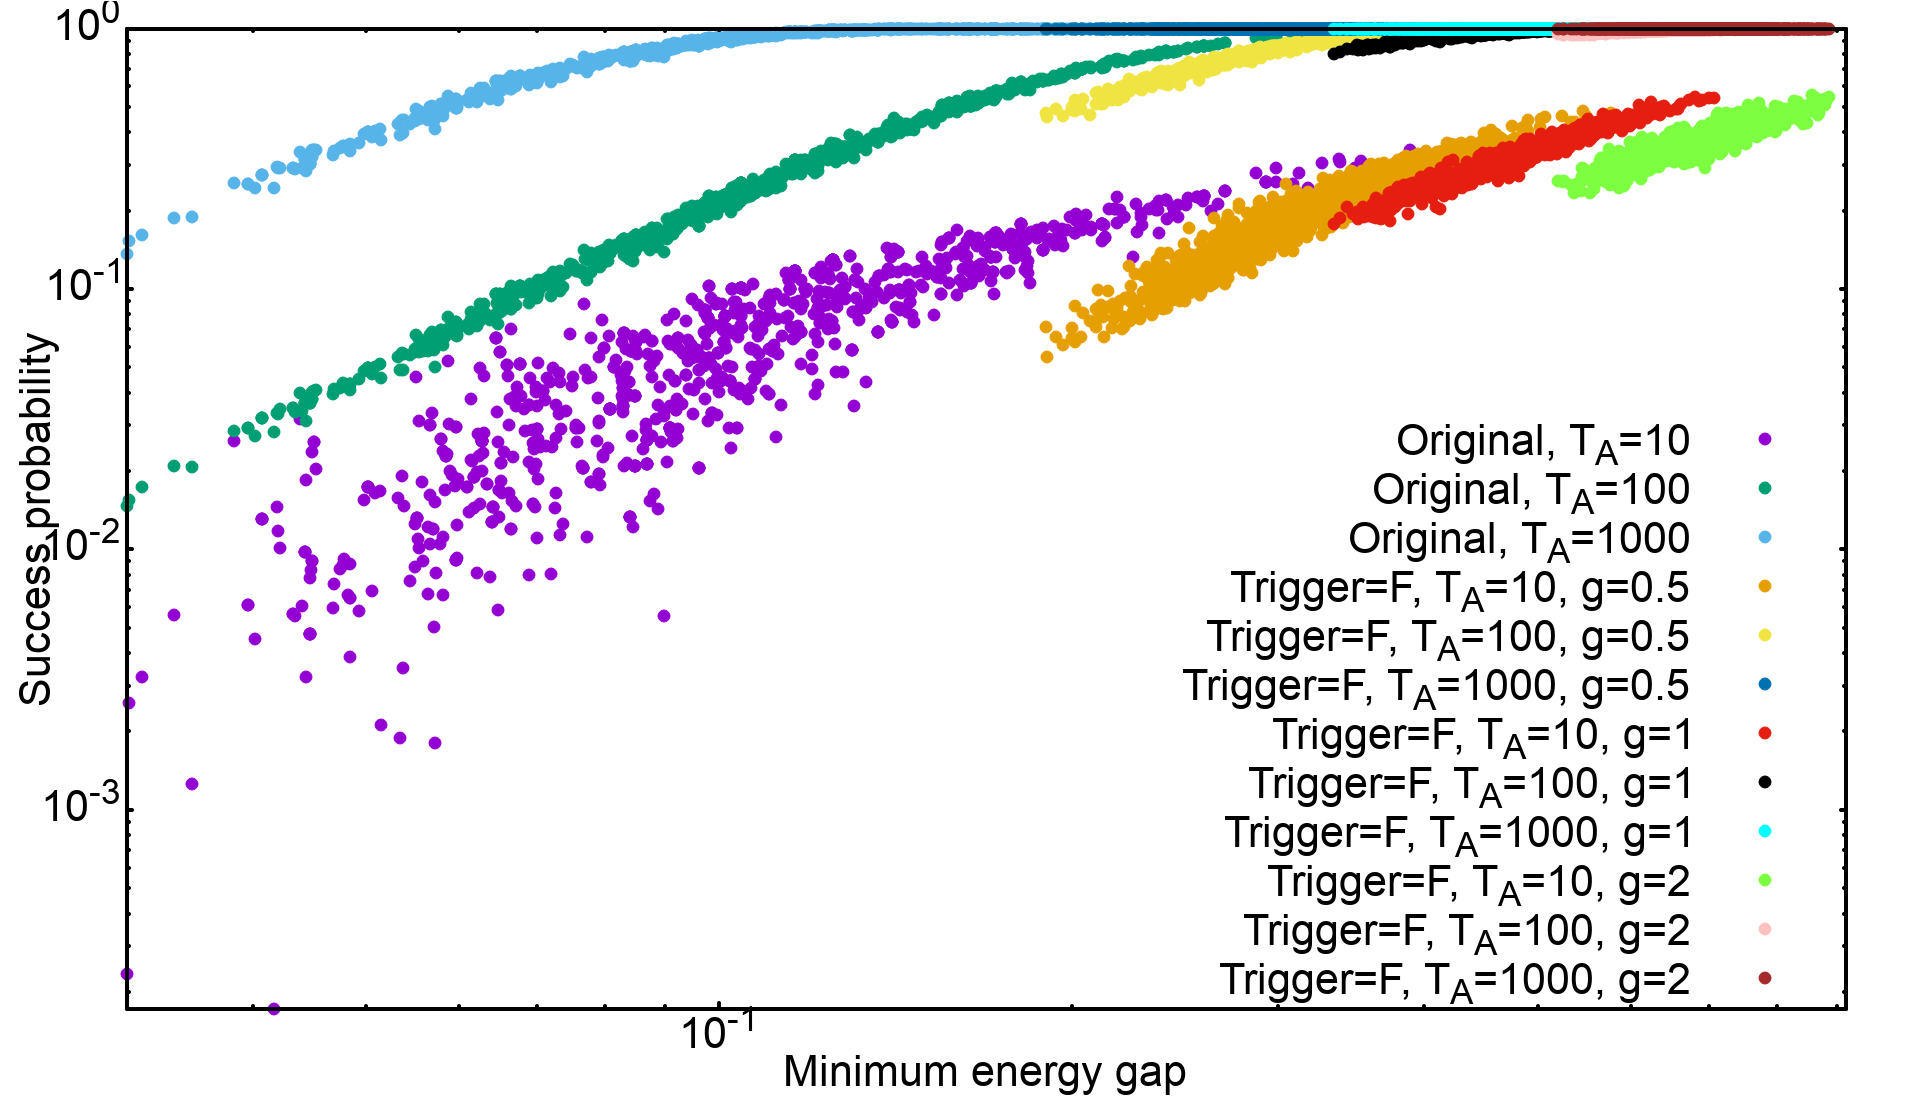
\includegraphics[scale=0.24]{SuccVsGap_OF_g.png}
\caption{Plot of the success probability versus minimum energy gaps for all the problems belonging to the set of the 12-variable 2-SAT problems. The plot shows the effect of adding ferromagnetic trigger to the original Hamiltonian with strengths 0.5, 1 and 2, while the annealing time is chosen to 10, 100 and 1000.}
\label{fig:f14}
\end{figure} 

From Fig.~(\ref{fig:f14}) it can be noted that all the curves roughly follow the Landau-Zener dependence (see Eq.~(\ref{eq:lz3})) of the success probability on the minimum energy gaps. However, for the original Hamiltonian, and $T_A$=10, the scattering is larger compared to the other curves. The scattering of the curves decreases on increasing the annealing times, suggesting that longer annealing times ascertain the evolution of the state to be closer to adiabatic. Since adding the ferromagnetic trigger enlarges the minimum energy gaps, the curves are shifted to the right upon adding the trigger and increasing their strength. 
\end{document}